\chapter{Hidden Markov Models}
\label{chapter:hmm}

This chapter introduces hidden Markov models (HMM), which are a widely
used model for POS tagging and morphological tagging. Extensions to
the HMM are further investigated in the next chapter and Publications
\ref{pub:1}, \ref{pub:2} and \ref{pub:3}.

\section{Example}
%\begin{itemize}
%\item Chained stochastic processes \citep{Rabiner1989}.
%\item The three classical problems of HMMs.
%\item Pioneered by \cite{Church1988} in POS tagging.
%\item The results by \cite{Brants2000} and \cite{Halacsy2007} probably
%  represent the generative state of the art.
%\item Very fast to train compared to discriminative models.
%\end{itemize}

I will illustrate Hidden Markov Models using an example. Imagine a
person called Jill who is hospitalized and occupies a windowless
room. The only way for her to know what is happening in the outside
world is to observe a nurse who passes her room daily.\footnote{To make things simple, imagine the nurse works every day.}

Suppose, Jill is interested in weather phenomena and she decides to
pass time by guessing if it is raining outside. She bases her guesses
on whether or not the nurse is carrying an umbrella. In other words,
she predicts an {\it unobserved variable}, the weather, based on an
{\it observed variable}, the nurse's umbrella.

There are several probabilistic models Jill might use. The simplest
useful model assigns probability $1$ to the event of rain, if the
nurse carries an umbrella, and assign it the probability $0$
otherwise. This simplistic model would certainly give the correct
prediction most of the time, but Jill believes that she can do better.

Jill knows that people often carry an umbrella when it is raining. She
also knows that they rarely carry one when the weather is
clear. However, people sometimes do forget their umbrella on
rainy days, perhaps because they are in a hurry. Moreover, people
sometimes carry an umbrella even when it is not raining. For example
the weather might be murky and they might anticipate rain. Therefore,
Jill decides to reserve some probability, say $0.2$, for the event
that the nurse is carrying an umbrella when there is no rain. She
reserves an equal probability for the event that the nurse arrives at
work without an umbrella although it is in fact raining.
 
Without additional information, this more complicated model will give
exactly the same MAP predictions as the simplistic one. Knowledge of
meteorology, however, also factors in. Let us suppose Jill is a
weather enthusiast and she knows that the probability of rain is
$0.25$ a priori, making the probability of clear weather $0.75$. She also knows
that the probability of rain increases markedly on days following
rainy days at which time it is $0.7$.  Similarly, the probability of
clear weather increases to $0.9$ if the weather was clear on the
previous day. Figure \ref{hmm-ex-1} summarizes these
probabilities.\footnote{Since the author of this thesis has very
  little knowledge about meteorology, these probabilities are likely
  to be nonsense. The overall probability of rain and clear weather
  is, however, chosen to be the steady state of the Markov chain
  determined by the probabilities of transitioning between
  states. Consistency is therefore maintained.}

\begin{figure}[!htb]
\begin{center}
\begin{tabular}{|l|c|}
\hline
   $\iota$   &       \\
\hline
CLEAR  & $0.75$ \\
RAIN  & $0.25$ \\
\hline
\end{tabular}~~~
\begin{tabular}{|l|cc|}
\hline
   $T$   & CLEAR & RAIN  \\
\hline
CLEAR  & $0.9$ & $0.1$ \\
RAIN   & $0.3$ & $0.7$ \\
\hline
\end{tabular}~~~
\begin{tabular}{|l|cc|}
\hline
   $E$   & 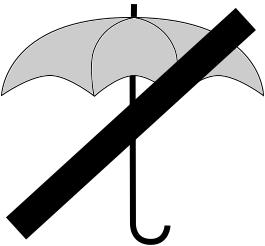
\includegraphics[width=0.5cm]{no_umbrella} & 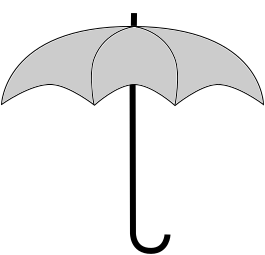
\includegraphics[width=0.5cm]{umbrella} \\
\hline
CLEAR   & $0.8$ &  $0.2$         \\
RAIN    & $0.2$ &  $0.8$         \\
\hline
\end{tabular}
\end{center}
\caption{The probability distributions which define the HMM in the
  weather forecast example. $\iota$ specifies the initial probability
  of CLEAR and RAIN. $T$ shows the transition distributions, which
  specify the probability of CLEAR and RAIN given the weather on the
  previous day. Finally, $E$ shows the emission distributions, which
  specify the probabilities of seeing an umbrella depending on the
  weather.}\label{hmm-ex-1}
\end{figure}

Let us assume that Jill observes the nurse for one week. She sees the
nurse carry an umbrella on all days except Tuesday. The MAP prediction
given by the simplistic model is that Tuesday is clear and all other
days are rainy. The more complex model will, however, give a different
MAP prediction: the probability is maximized by assuming that all days
are rainy. Under the more complex model, it is simply more likely that
the nurse forgot to bring an umbrella on Tuesday.

\begin{figure}[!htb]
\begin{center}
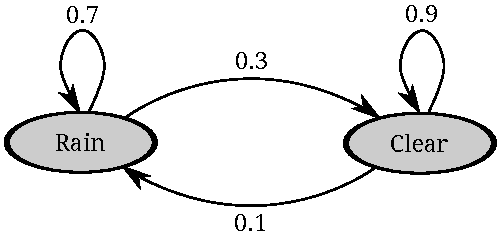
\includegraphics[scale=0.8]{hmm-ex-graph}
\caption{A visual representation of the HMM in Figure \ref{hmm-ex-1}.}\label{hmm-ex-2}
\end{center}
\end{figure}

The model Jill is using for weather prediction is called a Hidden
Markov Model. It can be used to make predictions about a series of
events based on indirect observations. 

The HMM is commonly visualized as a directed graph. Each hidden state,
for example RAIN and CLEAR, represents a vertex in the
graph. Transitions from one hidden state to another are represented by
arrows labeled with probabilities. Figure \ref{hmm-ex-2} shows a graph
representing the transition structure of the HMM outlined in Figure
\ref{hmm-ex-1}.

\section{Formal Definition}

%\begin{itemize}
%\item Model derivation.
%\item Lexical model.
%\item First order transition model.
%\item Model order.
%\item Guesser for OOV words à la Brants.
%\end{itemize}

Abstracting from the example above, an HMM is a probabilistic model
that generates sequences of state observation pairs. At each step $t$
in the generation process, the model generates an observation by
sampling the {\it emission distribution} $\varepsilon_{y_t}$ of the
current state $y_t$. It will then generate a successor state $y_{t+1}$
by sampling the {\it transition distribution} $\tau_{y_t}$ of state
$y_t$. The first hidden state $y_1$ is sampled from the {\it initial
  distribution} $\iota$ of the HMM.

Since the succession of days is infinite for all practical purposes,
there was no need to consider termination in the example presented in
Figure \ref{hmm-ex-2}. Nevertheless, many processes, such as sentences, do
have finite duration. Therefore, a special {\it final state} $f$ is
required. When the process arrives at the final state, it stops:
no observations or successor states are generated.

Following \cite{Rabiner1989}\footnote{The definition of HMMs in this
  thesis differs slightly from \cite{Rabiner1989} since I utilize
  final states.  }, I formally define a {\it discrete} HMM as a
structure $(Y,\ X,\ i,\ T,\ E,\ F)$ where:
\begin{enumerate}
\item $Y$ is the set of hidden states ($Y = \{{\rm CLEAR},$ ${\rm RAIN}\}$
  in the example in Figure \ref{hmm-ex-1}).
\item $X$ is the set of emissions, also called observations (
%$\Sigma =
%  \{{\rm Umbrella},$ ${\rm No\ umbrella}\}$ 
$X = \{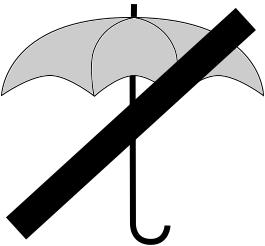
\includegraphics[width=0.4cm]{no_umbrella},\ 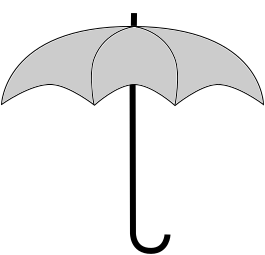
\includegraphics[width=0.4cm]{umbrella}\}$
in the example in Figure
  \ref{hmm-ex-1}).
\item $\iota: Y \rightarrow \R$ is the initial state distribution, that is the probability
  distribution determining the initial state of an HMM process (array
  $\iota$ in Figure \ref{hmm-ex-1}).
\item $T$ is the collection of transition distributions, $\tau_y: Y \rightarrow \R$, that
  determine the probability of transitioning from a state $y$ to each state
  $y' \in Y$ (array $T$ in Figure \ref{hmm-ex-1}).
\item $E$ is the collection of emission distributions $\varepsilon_y:
  X \rightarrow \R$, which determine the probability of observing each
  emission $o \in X$ in state $y \in Y$ (array $E$ in Figure
  \ref{hmm-ex-1}).
\item $f \in Y$ is the final state. The state $f$ emits no
  observations and there are no transitions from $f$.
\end{enumerate}

Figure \ref{hmm-ex-3} gives a visualization of the HMM in Figure \ref{hmm-ex-1} with an added final state. 
Because the progression of days is infinite for all practical purposes, the
probability of transitioning to the final state $f$ in example
\ref{hmm-ex-2} is 0 regardless of the current state. Hence, the
probability of any single sequence of states and emissions is
0. The probability of an initial segment of a state sequence
may, however, be non-zero.\footnote{The probability of an initial segment
  up to position $t$ can be computed using the forward algorithm,
  which is presented in Section \ref{sec:forward}.}% For example, the
%probability that the first three states are (RAIN, RAIN, CLEAR) is X.

\begin{figure}[!htb]
\begin{center}
\caption{Foo}\label{hmm-ex-3}
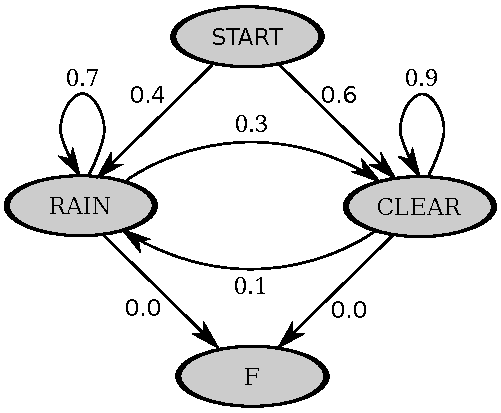
\includegraphics[scale=0.8]{hmm-ex-graph-2}
\end{center}
\end{figure}

An HMM models a number of useful quantities:
\begin{enumerate}
\item The {\it joint probability} $p(x,y\parcond\theta)$ of a observation
  sequence $x$ and state sequence $y$. This is the probability that an
  HMM with parameters $\theta$ will generate the state sequence $y$
  and generate the observation $x_t$ in every state $y_t$.
\item The {\it marginal probability} $p(x\parcond \theta)$ of an
  observation sequence $x$. This is the overall probability that the
  observation sequence generated by an HMM is $x$.
\item The {\it conditional probability} $p(y\cond x\parcond\theta)$ of a
  state sequence $y$ given an observation sequence $x$. That is, how
  likely it is that the model passes through the states in $y$ when
  emitting the observations in $x$ in order.
\item The {\it marginal probability $p(z, t,\ x\parcond \theta)$ of
    state $z$ at position $t$} when emitting the observation sequence
  $x$. That is, the probability of emitting observation sequence $x$
  under the single constraint that the state at position $t$ has to be $z$.
\end{enumerate}

To formally define these probabilities, let $\theta = \{\iota,\ T,\
E\}$ be the parameters of some HMM with observation set $X$ and hidden
state set $Y$, $x \in X^T$ be a sequence of
observations and $y \in Y^{T+1}$ a sequence of
hidden states. The last state $y_{T+1}$ in $y$ has to be the final state
$f$. Then the joint probability $p(x,y\parcond\theta)$ of $x$ and $y$
given $\theta$ is defined by Equation \eqref{hmm-joint-prob}.
\begin{equation}
p(x,y\parcond\theta) = p(y\parcond\theta)\cdot p(x \cond y\parcond\theta)= \Bigg(\iota(y_1) \cdot \prod_{t = 1}^{T} \tau_{y_t}(y_{t + 1})\Bigg) \cdot \prod_{t = 1}^T \varepsilon_{y_t}(x_t)\label{hmm-joint-prob}
\end{equation}
Equation \eqref{hmm-joint-prob} is a product of two factors: the
probability of the hidden state sequence $y$, determined by the
initial and transition probabilities, and the probability of the
emissions $x_t$ given hidden states $y_t$ determined by the emission
probabilities.

%FIXME: Talk about language models and stuff.
When the HMM model is used as a morphological tagger, the emissions
are word forms and the hidden states are morphological labels. This
allows for capturing simple grammatical dependencies between adjacent
morphological labels. For example, in English, a determiner is often
followed by an adjective, participle, noun or adverb, but rarely
followed by an active verb form or another determiner. The HMM can,
therefore, be seen as a simple probabilistic model of grammar
where the grammar rules only concern co-occurrences of words and
labels as well as co-occurrences of adjacent labels. As demonstrated
by the success of the HMM model in POS tagging, this simple model can
be surprisingly effective.

In the standard HMM, every hidden states in $Y$ has a probability for
emitting any given observation (of course, the emission probability
for a particular observation can be zero in some states). Therefore,
several state sequence $y \in Y^{T+1}$ can be generate the same
sequence of observations $x \in X^T$. The marginal probability
$p(x\parcond\theta)$ of an observation sequence $x$ can be found by
summing over all state sequences that could have generated $x$. It is
defined by Equation \eqref{hmm-obs-prob}.
\begin{equation}
p(x\parcond\theta) = \sum_{y \in Y^{T+1},\ y_{T+1} = f} p(x, y\parcond \theta)\label{hmm-obs-prob}
\end{equation}

Possibly the most important probability associated to the HMM is the
conditional probability $p(y\cond x\parcond\theta)$ of state sequence $y$
given observations $x$. This is an important quantity because
maximizing $p(y\cond x\parcond\theta)$ with regard to $y$ will give the MAP
assignment of observation sequence $x$. It is defined by Equation
\eqref{hmm-cond-prob}.
\begin{equation}
p(y\cond x\parcond\theta) = \frac{p(x,y\parcond\theta)}{p(x\parcond\theta)}\label{hmm-cond-prob}
\end{equation}
It is noteworthy, that $p(y\cond x\parcond\theta) \propto p(x,y\parcond\theta)$ because the marginal probability $p(x\parcond\theta)$ is independent of $y$. Therefore, $y$ maximizes $p(y\cond x\parcond\theta)$ if and only if, it maximizes $p(x,y\parcond\theta)$. This facilitates inference because the MAP assignment for the hidden states can be computed without computing the marginal probability $p(x\parcond\theta)$.

Finally, the posterior marginal probability of state $z$ at position $t$ given
the observation sequence $x$ is computed by summing, or marginalizing,
over all state sequence $y$, where $y_t = z$. It is defined by
Equation \eqref{hmm-marg-prob}
\begin{equation}
p(z, t,\ x\parcond \theta) = \sum_{y' \in Y^{T+1},\ y'_t = z,\ y'_{T+1} = f} p(x, y'\parcond \theta)\label{hmm-marg-prob}
\end{equation}

\section{Inference}
%\begin{itemize}
%\item The forward algorithm.
%\item Guarding against underflow: Dynamic scaling \citep{Rabiner1989} or exp-sum-log \citep{Durbin1998}.
%\item The Viterbi algorithm.
%\item Fixed beam search.
%\item Determining the beam: fixed, threshold and adaptive beam \citep{pal2006}.
%\item The forward-backward algorithm and multitagging.
%\end{itemize}
Informally, inference in HMMs refers to finding a maximally
probable sequence of hidden states $y$ that might have emitted the
observation $x$. As \cite{Rabiner1989} points out, this statement is
not strong enough to suggest an algorithm. 

Maximally probable is an ambiguous term when dealing with structured
models. It could be taken to mean at least two distinct things. The
MAP assignment $y_{MAP}$ of the hidden state sequence is the most
probable joint assignment of states defined by Equation
\eqref{hmm-map} and depicted in Figure
\ref{hmm-ex-trellis-path}. 
\begin{equation}
y_{MAP} = \argmax_{y\in Y^T} p(y\cond x\parcond\theta)\label{hmm-map}
\end{equation}

Another possible definition would be the
{\it maximum marginal} (MM) assignment. It chooses the most probable
hidden state for each word considering all possible assignments of states for the remaining words. The MM assignment $y_{MM}$ is defined by Equation
\eqref{hmm-mm}. Figure \ref{hmm-ex-trellis-marginal} shows the
paths whose probabilities are summed in order to compute the marginal for one position and state.


\begin{equation}
y_{MM} = \argmax_{y\in Y^T} \prod_{t = 1}^T p(y_t, t \cond x\parcond\theta)\label{hmm-mm}
\end{equation}

As \cite{Merialdo1994} and many others have noted, the MAP and MM
assignments maximize different objectives. The MM assignment maximizes
the accuracy of correct states per observations whereas the MAP
assignment maximizes the number of completely correct state
sequences. Both objectives are important from the point of view of POS
tagging in a theoretical sense. However, they are often quite
correlated and, at least in POS tagging, it does not matter in
practice which of the criteria is used \citep{Merialdo1994}. Most
systems, for example \cite{Church1988,Brants2000,Halacsy2007}, have
chosen to use MAP inference, possibly because it is easier to
implement and faster in practice.

Although, MM inference is more rarely used with HMMs, computing the
marginals is important both in unsupervised estimation of HMMs and
discriminative estimation of sequence models. Therefore, an efficient
algorithm for MM inference, the {\it forward-backward algorithm}, is presented below.

There are a number of strongly related algorithms for both exact MAP
and MM inference. The work presented in this thesis, uses the Viterbi
algorithm for MAP inference and the forward-backward algorithm for MM
inference \citep{Rabiner1989}. {\it Belief propagation}, introduced by
\cite{Pearl1982}, computes the MM assignment and can be modified to
compute the MAP assignment as well. For sequence models, such as the
HMM where hidden states form a directed sequence, belief propagation
is very similar to the forward-backward algorithm. It can, however, be
extended to cyclic graphs \citep{Weiss2000} unlike the Viterbi
algorithm.

Since cyclic models fall beyond the scope of this thesis and both the
Viterbi and forward-backward algorithms are amenable to well known
optimizations, which are of great practical importance, I will not
discuss belief propagation further. \cite{Koller2009} gives a nice
treatment of belief propagation and graphical models at large.

Before introducing the Viterbi and forward-backward algorithm, it is
necessary to investigate the forward algorithm, which is used to
compute the marginal probability of an observation and also as part of
the forward-backward algorithm. The forward algorithm and Viterbi
algorithm are closely related.

\begin{figure}[!p]
\begin{center}
\caption{foo.}\label{hmm-trellis}
\begin{subfigure}{\textwidth}
\begin{center}
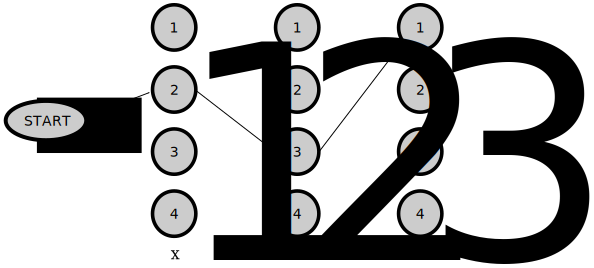
\includegraphics[scale=0.65]{trellis_path}
\caption{Trellis and path.}\label{hmm-ex-trellis-path}
\end{center}
\end{subfigure}
\vskip.5cm
\begin{subfigure}{\textwidth}
\begin{center}
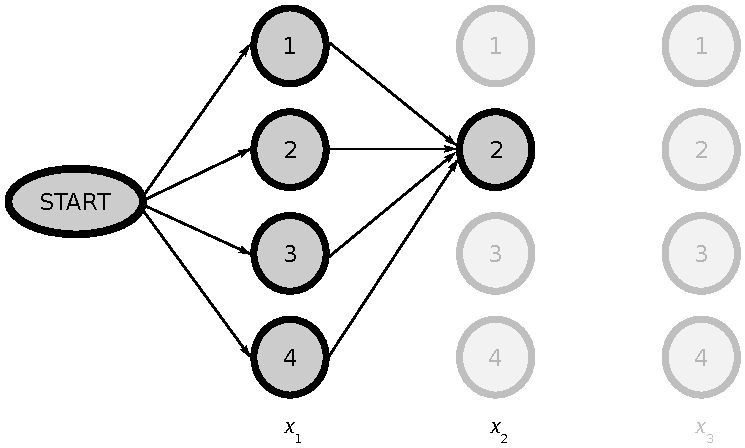
\includegraphics[scale=0.65]{trellis_forward}
\end{center}
\caption{Forward path prefixes.}\label{hmm-ex-trellis-fw}
\end{subfigure}
\vskip.5cm
\begin{subfigure}{\textwidth}
\begin{center}
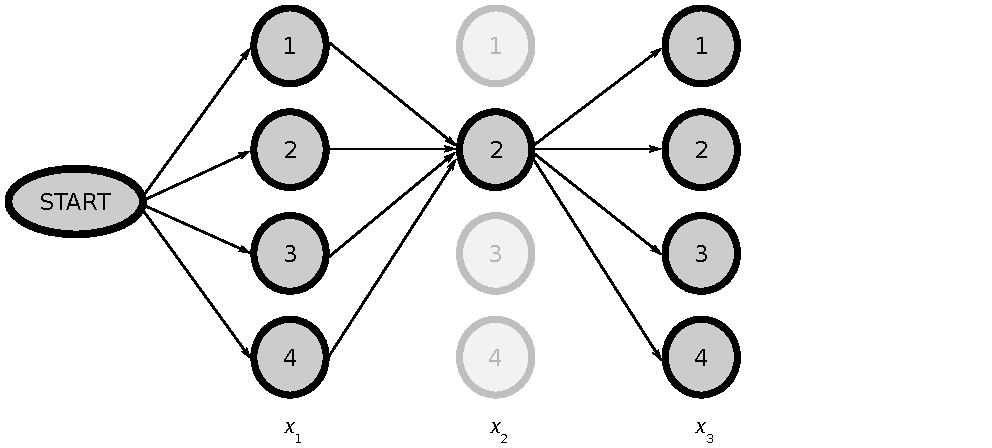
\includegraphics[scale=0.65]{trellis_marginal}
\end{center}
\caption{Marginal paths.}\label{hmm-ex-trellis-marginal}
\end{subfigure}
\end{center}
\end{figure}

\paragraph{The Forward Algorithm}
\label{sec:forward}
Equations \eqref{hmm-map} and \eqref{hmm-mm} reveal, that both MAP
and MM inference require knowledge of the entire observation $x$. In
the weather prediction example, observations are, however, always
infinite. What kind of inference is possible in this case?

Even when we only know a prefix $x[1:t]$ (of length $t$) of the entire
observation $x$, we can still compute the {\it belief state}
\citep{Boyen1998} of the HMM given the prefix. The belief state is in
fact not a single state, but rather a distribution over the set of
hidden states $Y$. It tells us how likely we are to be in state $z$ at
time $t$, when we have emitted the prefix $x[1:t]$.

To compute the belief state at position $t$, we first need to compute
the {\it forward probabilities} for each state $z \in Y$. The forward
probability $\fw_{t,z}(x)$ of state $z$ at position $t$ is the
probability of emitting prefix $(x_1, ..., x_t)$ and ending up in state $z \in
Y$. For example, given an infinite observation 
%$x = (${\sc umbrella},
%{\sc umbrella}, {\sc no umbrella},\ ...$)$
$(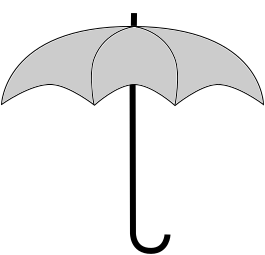
\includegraphics[width=0.4cm]{umbrella},\ 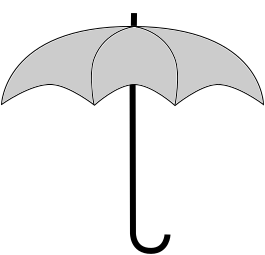
\includegraphics[width=0.4cm]{umbrella},\ 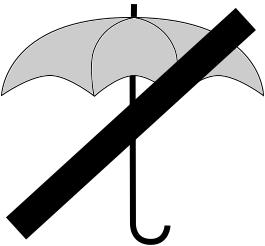
\includegraphics[width=0.4cm]{no_umbrella},\ ...)$, the forward probability
$\fw_{3,\textsc{RAIN}}$ is the probability that the third day is rainy,
when the nurse carried an umbrella on the first and second days, but
did not carry one on the third day.

I am going to make a technical but useful definition. The {\it prefix probability} of observation sequence $x = (x_1,\ ...,\ x_T)$ and state sequence $y = (y_1,\ ...,\ y_t)$ at position, where $t < T + 1$ is given by Equation \eqref{prefix_prob}. 
\begin{equation}
p(x,\ y\parcond \theta) = \Bigg(\iota(y_1) \cdot \Bigg(\prod_{u = 1}^{t - 1} \tau_{y_u}(y_{u + 1}) \Bigg) \cdot \prod_{u = 1}^t \varepsilon_{y_u}(x_u)\Bigg),\ t \le T\label{prefix_prob}
\end{equation}
When $t = T$, this is almost the same as the joint probability of $x$ and
$y$, but the final transition is missing.

Conceptually, the forward probability is computed by summing over the
probabilities of all path prefixes up to position $t$, where the state
at position $t$ is $z$, see Figure \ref{hmm-ex-trellis-fw}. Formally,
the forward probability is defined by Equation \eqref{forward_prob}.
\begin{equation}
\fw_{t,z} = \sum_{y\in Y^t,\ y_t = z} p(x,\ y\parcond\theta)\label{forward_prob}
\end{equation}
Comparing Equations \eqref{forward_prob} and \eqref{hmm-joint-prob}
shows that the forward probability in a sense represents the
probability of a prefix of observation $x$.

The belief state and posterior marginal distribution may seem
similar. They are, however, distinct distributions because the belief
state disregards all information about observation $x$ after position
$t$. In contrast, the marginal distribution encompasses information
about the entire observation. For example the marginal probability of
RAIN at position 3 is likely to depend strongly on whether or not Jill
observes the nurse carry an umbrella on the fourth day. However, this
will have no impact on the belief state.

Figure \ref{fw-naive-prob} demonstrates a naive approach to computing
the forward probabilities. Simply list all relevant state sequences,
compute the probability of each sequence and sum the
probabilities. Unfortunately, the naive approach fails for large $t$
because the number of distinct state sequences depends on the sequence
length in an exponential manner.

The complexity of the naive algorithm is $|Y|^t$, which is infeasible.
For example, $f_{20,\textsc{RAIN}}(x)$ requires us to sum
approximately 20 million probabilities and $f_{30,\textsc{RAIN}}(x)$
entails summation of approximately 540 million probabilities. Since
observation sequences in domains such as natural language processing
frequently reach lengths of $100$, a more efficient approach is required.

\begin{figure}[!ftb]
\begin{center}
\caption{A naive approach to computing forward probabilities.}\label{fw-naive-prob}
\begin{tabular}{lllr}
$y_1$ & $y_2$ & $y_3$ & $p$ \\
\hline
{\sc CLEAR} & {\sc CLEAR} & {\sc CLEAR} & $(0.75\cdot0.8\cdot0.9\cdot0.2)\cdot0.9\cdot0.8\approx0.078$\\
{\sc RAIN}  & {\sc CLEAR} & {\sc CLEAR} & $(0.25\cdot0.2\cdot0.3\cdot0.2)\cdot0.9\cdot0.8\approx0.002$\\
{\sc CLEAR} & {\sc RAIN}  & {\sc CLEAR} & $(0.75\cdot0.8\cdot0.1\cdot0.8)\cdot0.3\cdot0.8\approx0.012$\\
{\sc RAIN}  & {\sc RAIN}  & {\sc CLEAR} & $(0.25\cdot0.2\cdot0.7\cdot0.8)\cdot0.3\cdot0.8\approx0.007$\\
& & & \\
%\hline
%\vspace{0.1cm}
~~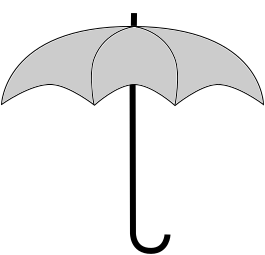
\includegraphics[width=0.5cm]{umbrella} & ~~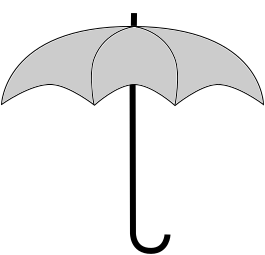
\includegraphics[width=0.5cm]{umbrella} & ~~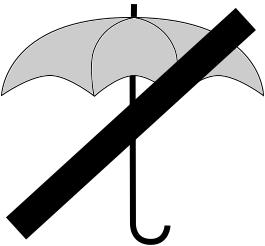
\includegraphics[width=0.5cm]{no_umbrella} & \\
\hline
        &       & & $\approx0.098$
\end{tabular}
\end{center}
\end{figure}

The belief state can be computed in linear time with regard to $t$ and
quadratic time with regard to $|Y|$ using the {\it forward algorithm}
\citep{Rabiner1989}, which is in fact simply a recursive application
of the right distributive rule of algebra
$$a_1 \cdot b + ... + a_n \cdot b = (a_1 + ... + a_n)\cdot b$$
for real numbers $a_1$ up to $a_n$ and $b$. 

Instead of computing the probability separately for each path, the
forward probabilities for longer paths are computed incrementally
using the forward probabilities of shorter paths. Examine Figure
\ref{fw-naive-prob}. By grouping rows one and two, as well as three
and four into pairs, it is easy to see that
$$\fw_{3,\textsc{CLEAR}} = (\fw_{2, \textsc{RAIN}}\cdot \tau_{\textsc{RAIN}}(\textsc{CLEAR}) + \fw_{2, \textsc{CLEAR}} \cdot \tau_{\textsc{CLEAR}}(\textsc{CLEAR})) \cdot \varepsilon_{\textsc{CLEAR}}(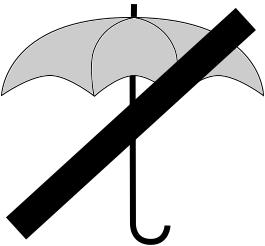
\includegraphics[width=0.4cm]{no_umbrella})$$
Generalizing, we get the recursion in Equation \eqref{fw-rec}.
\begin{equation}
\fw_{t, z} = \left\{
\begin{aligned}
&\iota(z) \cdot \varepsilon_{z}(x_1)  & , &\  t = 1\\
&\Bigg(\sum_{z'\in Y} \fw_{t - 1, z'}\cdot \tau_{z'}(z) \Bigg) \cdot \varepsilon_{z}(x_{t}) & ,&\ 1 < t \le T\\
&\sum_{z'\in Y} \fw_{T, z'}\cdot \tau_{z'}(f) & ,&\  t = T + 1,\ z = f.
\end{aligned}
\right.
\label{fw-rec}\end{equation}
The remaining forward probabilities $\fw_{T+1, z}$, where $z \ne f$
are defined to be $0$.

The forward probability $f_{T + 1, f} = p(x \parcond \theta)$. In fact
one of the principal applications for the forward algorithm is
computing the marginal probability of an observation. The other
central application is in the forward-backward algorithm, which
computes the state marginals.
  
The forward algorithm is outlined in Algorithm
\ref{forward-algorithm}. Assuming that accessing the data structures
{\tt x}, {\tt i_prob}, {\tt e_prob}, {\tt tr_prob} and {\tt trellis}
is constant time, the complexity of the algorithm is dominated by the
three nested loops on lines \ref{start-cplx}--\ref{stop-cplx}. This
shows that the complexity of the forward algorithm is linear with
regard to the length of the sequence and quadratic with regard to the
size of the hidden state set.

Although, the forward algorithm depends linearly on the observation
length, its quad\-ra\-tic dependence on the size of the hidden state set
is problematic from the perspective of morphological disambiguation of
morphologically complex languages, where the size of the hidden state
set is measured in the hundreds or thousands for regular HMMs. When
using second order HMMs presented below, the state set can grow to
tens of thousands or millions, which can slow down systems to a degree
that makes them infeasible in practice. I will present partial
solutions to these problems below.

\begin{algorithm}[!p]
\begin{center}
\caption{The forward algorithm in Python 3.}\label{forward-algorithm}
\begin{lstlisting}[linewidth=\textwidth]
def forward(x, i_prob, e_prob, tr_prob): 
    """
        x       - The observation as a list.
        i_prob  - Initial state distribution.
        e_prob  - Emission distributions.
        tr_prob - Transition distributions.

        Return the trellis of forward probabilities. 
    """

    assert(not x.empty()) 

    trellis = {}

    # Indexing in python starts at 0.
    x_1 = x[0]
    T   = len(x) + 1

    # Set final state F. States are consecutive integers 
    # in the range [0, F]. 
    F = len(i_prob) - 1 

    # Initialize first trellis column.
    for z in range(F):
        trellis[(1,z)] = i_prob[z] * e_prob[z][x_1]

    # Set all except the final column.(*@\label{start-cplx}@*)
    for t in range(2, T):
        trellis[(t, z)] = 0

        x_t = x[t - 1]

        for z in range(F):
            for s in range(F):
                trellis[(t, z)] = trellis[(t - 1, s)] * tr_prob[s][z]

            trellis[(t, z)] *= em_prob[z][x_t](*@\label{stop-cplx}@*)

    # Set the last column.
    for z in range(s_count):
        trellis[(T + 1, z)] = trellis[(T, z)] * tr_prob[z][F]

    return trellis 
\end{lstlisting}
\end{center}
\end{algorithm}

\paragraph{The Viterbi Algorithm}
\label{hmm-viterbi}
Whereas the forward algorithm incrementally computes the marginal
probability of an observation $x$, the Viterbi algorithm incrementally
computes the MAP assignment for observation $x$.

A naive approach to finding the MAP assignment is to list all the
hidden state paths, compute their probabilities and pick the one with
the highest probability. Similarly as for the forward algorithm, the
complexity of this approach is exponential with regard to the length
of observation $x$.

Just as in the case of forward probabilities, the MAP assignment of
hidden states for a prefix of the observation $x$ can be computed
incrementally. Formally, the MAP assignment for a prefix $x[1:t]$ is
defined by equation \eqref{map_prefix} utilizing the joint prefix
probability of $x$ and a state sequence $y$ of length
$t$. Intuitively, it is the sequence of hidden states $y_{t, z}$ which
maximizes the joint probability and ends at state $z$.
\begin{equation}
y_{t,z} = \argmax_{y\in Y^t,\ y_t = z} p(x,\ y\parcond \theta)\label{map_prefix}
\end{equation}
Comparing this equation with the definition of the forward probability
$f_{t,z}$ in Equation \ref{forward_prob}, we can see that the only
difference is that the sum has been changed to $\argmax$.

I will now show that the MAP prefix $y_{t,z}$ can be computed
incrementally in a similar fashion as the forward probability
$f_{t,z}$. Suppose that $y_{t+1, z'} = (y_1,\ ...,\ y_t = z,\ y_{t+1}
= z')$. I will show that $y_{t+1, z'}[1:t] = y_{t,z}$. Let $y'$ be the concatenation of $y_{t,z}$ and $z'$. If $y_{t+1,z'}[1:t] \ne y_{t,z}$, then
\begin{eqnarray*}
p(x,\ y_{t+1,z'}\parcond \theta) & = & p(x,\ y_{t+1,z'}[1:t]\parcond \theta) \cdot \tau_z(z')\cdot\varepsilon_{z'}(x_{t+1})\\ 
                                 & < & p(x,\ y_{t,z}\parcond \theta) \cdot \tau_z(z')\cdot\varepsilon_{z'}(x_{t+1})\\
                                 & = & p(x, y'\parcond\theta)
\end{eqnarray*}
This contradicts the definition in Equation \eqref{map_prefix}.\footnote{As long as we suppose that there is exactly one MAP prefix.}

We now get Equation \eqref{map-rec}, which gives us a recursion. The
implementation of the Viterbi algorithm is identical to the
implementation of the forward algorithm except that sums are replaced
by maximization. Consequently, the time complexity of the algorithm is the
same. It is linear with regard to sentence length and quadratic with
regard to the size of the state set.
\begin{equation}
y_{t+1, z} = \argmax_{z \in Y}\left\{
\begin{aligned}
&\iota(z) \cdot \varepsilon_{z}(x_1)  & , &\  t = 1\\
&y_{t - 1, z'}\cdot \tau_{z'}(z) \cdot \varepsilon_{z}(x_{t}) & ,&\ 1 < t \le T\\
&y_{T, z'}\cdot \tau_{z'}(f) & ,&\  t = T + 1,\ z = f.
\end{aligned}
\right.
\label{map-rec}
\end{equation}

\paragraph{Beam Search}
As seen in the previous section, the complexity of the Viterbi
algorithm depends on the square of the size of the hidden state
set. This can be problematic when the set of hidden states is large,
for example when the states represent morphological labels in a very large label
set or when they represent combinations of labels. When tagging, a
morphologically complex language, the state set may easily encompass
hundreds or even thousands of states.

{\it Beam search} is is a heuristic which prunes the search space
explored by the Viterbi algorithm based on the following observation:
in many practical applications, the number of hidden states, which emit
a given observation with appreciable probability, is small. This is
true even when the total number of hidden states is very large. For
example, when the states represent morphological labels, a given word such as
``dog'' can usually only be emitted by a couple of states (maybe Noun
and Verb in this case).

When the Viterbi algorithm maximizes \eqref{map-rec} for $y_{t+1,z}$,
a large number of histories $y_{t,z}$ can, therefore, be ignored.

Often a constant number, the {\it beam width}, of potential histories
are considered in the maximization. The complexity of the Viterbi
algorithm with beam search is $o(|x||b||\mathcal{Y}|)$, where $|x|$ is the input length, $|b|$ the beam width and $|\mathcal{Y}|$ the size of the state set.
\footnote{Sequential decoding, an approximate inference
  algorithm, which was used for decoding before the Viterbi algorithm
  was in common use \citep{Forney2005} is very similar to beam
  search. Indeed, it could be said that Viterbi invented an exact
  inference algorithm, which is once more broken by beam search.}

In addition to histories, the possible hidden states for output can
also be filtered. The simplest method in to use a so called tag
dictionary. These techniques are described in Section
\ref{sec:hmm-label-dict}.

\paragraph{The Forward-Backward Algorithm}
\label{hmm-fw-bw}
The Viterbi algorithm computes the MAP assignment for the hidden
states efficiently. For efficiently computing the marginal probability
for a every state and position (see Figure
\ref{hmm-ex-trellis-marginal}), the forward-backward algorithm is
required.

Intuitively, the probability that a state sequence $y$ has state $z \in Y$
at position $t$, that is the probability that $y_t = z$, is the product
of the probabilities that the prefix $y[1:t]$ ends up at state $z$ and
the probability that the suffix $y[t:T]$ originates at $z$. 

The name forward-backward algorithm stems from the fact, that the
algorithm essentially consists of one pass of the forward algorithm,
which computes prefix probabilities, and another pass of the forward
algorithm starting at the end of the sentence and moving towards the
beginning which computes suffix probabilities. Finally, the forward
and suffix probabilities are combined to give the marginal probability
of all paths where the state at position $t$ is $z$. These passes are
called the forward and backward pass, respectively.

Formally, the suffix probabilities computed by the backward pass are
defined by equation \eqref{bw-rec}.

Since a backward pass of the forward algorithm carries the same
complexity as the forward pass, we can see that the complexity of the
forward-backward algorithm is the same as the complexity of the
forward algorithm, however, there is a constant factor of two compared
to the forward algorithm.

\begin{equation}
b_{t, z} = \left\{
\begin{aligned}
&\Bigg(\sum_{z'\in Y}t_{z}(z') \cdot  b_{t + 1, z'} \Bigg) \cdot e_{z}(x_{t+1}) & ,&\ 1 < t < T\\
&t_{z}(f) & ,&\  t = T + 1,\ z = f.
\end{aligned}
\right.
\label{bw-rec}
\end{equation}

%\paragraph{Sparse Forward-Backward Algorithms}
%FIXME \citep{Pal2006}.

\section{Estimation}
%\begin{itemize}
%\item Counting vs Baum-Welch.
%\item Smoothing over orders.
%\item Smoothing missing counts.
%\item Estimating parameters for OOV word model.
%\end{itemize}

HMMs can be trained in different ways depending on the quality of the
available data, but also on the task at hand. The classical setting
presented by \cite{Rabiner1989} is nearly completely unsupervised: the
HMM is trained exclusively from observations. Some supervision is
nevertheless usually required to determine the number of hidden
states.\footnote{Although methods for determining the number of states
  from the data exist \citep{foo}.} Additionally priors on the
emission and transitions distributions may be required to avoid
undesirably even distributions
\citep{Cutting1992,Johnson2007}.

The unsupervised training setting has two important and
interrelated applications:
\begin{enumerate}
\item Modeling a complex stochastic process from limited data. Here
  the HMM can be contrasted to a Markov chain \citep[318--320]{Manning1999}, where
  each emission can occur in a unique state leading to a higher degree
  of data sparsity and inability to model under-lying structure.
\item Uncovering structure in data, for example part-of-speech
  induction \citep{Johnson2007}.
\end{enumerate}
The classical method for unsupervised Maximum likelihood estimation of
HMMs is the {\it Baum-Welch algorithm} \citep{Rabiner1989}, which is
an instance of the {\it expectation maximization algorithm} (EM)
\citep{Dempster1977} for HMMs.

In morphological tagging, the supervised training scenario is normally
used. Supervised training consists of annotating a text corpus with
POS labels and estimating the emission and transition probabilities
from the annotated data.

Straight-forward counting is sufficient to get the ML estimates for
the transition and emission distributions. For example, one can simply
count how often a determiner is followed by a noun, an adjective or
some other class. Similarly, one can count how many often a verb label
emits ``dog'' and how often the noun label emits ``dog''. 

Even in large training corpora, ``dog'' might very well never receive
a verb label.\footnote{There are ten occurrences of ``dog'' in the Penn
  Treebank and all of them are analyzed as nouns.} Nevertheless,
``dog'' can be a verb, for example in the sentence ``Fans may dog
Muschamp, but one thing's for certain: he did things the right way off
the field.''. To avoid this kind of problems caused by data sparsity,
both emission and transition counts need to be smoothed.

\paragraph{Counting for Supervised ML Estimation}\label{sec:hmm-counting}
When HMMs are used in linguistic labeling tasks, such as
part-of-speech tagging, they are usually estimated in a supervised
manner. Each label is thought to represent a hidden variable, and the
HMM models the transitions from one label type to another and the
emission of words from each label type. 

\begin{figure}[!htb]
\begin{center}
\begin{BVerbatim}
Mr.             NNP
Vinken          NNP
is              VBZ
chairman        NN
of              IN
Elsevier        NNP
N.V.            NNP
,               ,
the             DT
Dutch           NNP
publishing      VBG
group           NN
.               .
\end{BVerbatim}
\end{center}
\caption{Tagged text from the Penn Treebank.}\label{penn-figure}
\end{figure}

Figure \ref{penn-figure} shows one sentence from the Penn Treebank \citep{Marcus1993}. The sentence is labeled with POS tags which are taken to be the hidden states of an HMM. When estimating an HMM tagger for the corpus, transitions probabilities, for example $t_{{\tt NNP}, {\tt VBZ}}$, and emission probabilities, for example $e_{{\tt NNP}}({\tt Dutch})$ can in principle be computed directly from the corpus. For example the transition probability $t_{{\tt NNP}, {\tt VBZ}}$ and the emission probability $e_{{\tt NNP}}({\tt Dutch})$ in the Penn Treebank are simply:
$$t_{{\tt NNP}, {\tt VBZ}} = \frac{{\rm Count\ of\ POS\ tag\ pair\ {\tt NNP}\ {\tt VBZ}\ in\ the\ corpus}}{{\rm Count\ of\ POS\ tag\ {\tt NNP}\ in\ the\ corpus}} = \frac{4294}{114053} \approx 0.04$$

$$e_{{\tt NNP}}({\tt Dutch}) = \frac{{\rm Number\ of\ times\ {\tt Dutch}\ was\ tagged\ {\tt NNP}\ in\ the\ corpus}}{{\rm Count\ of\ POS\ tag\ {\tt NNP}\ in\ the\ corpus}} = \frac{14}{114053} \approx 1.2 \cdot 10^{-4}$$

Simple computation of co-occurrences is insufficient because of
data-sparsity. Words do not occur with all POS tags in the training
corpus and all combinations of POS tags are never observed. Sometimes
this is not a problem. For example, ``Dutch'' could never be a
preposition. We know that the probability that a preposition state
emits ``Dutch'' is $0$. However, there are at least three analyses
that are perfectly plausible: noun (the Dutch language), adjective
(property of being from The Nederlands) and proper noun (for example
in the restaurant name ``The Dutch'').

Since ``Dutch'' occurs only 14 times in the Penn Treebank, it is not
surprising that all of these analyses do not occur. Specifically, the
noun analysis is missing. An HMM based on direct counts will therefore
never analyze ``Dutch'' as a noun.

It is tempting to think that missing analyses are a minor problem
because they only occur for relatively rare words such as
``Dutch''. Unfortunately, a large portion of text consists of rare
words. The problem therefore has very real consequences.

The usual approach is to use a family of techniques called {\it
  smoothing}. In smoothing, zero counts and all other counts are
modified slightly to counter-act sparsity.

Smoothing of emission probabilities and transition probabilities differ
slightly. For transition probabilities it is common practice to use
counts of both tag pairs and single tags to estimate tag probabilities
either in a back-off scheme or using interpolation
\citep{Brants2000}. %Many sophisticated interpolation schemes can be
%used for example Kneser-Ney \citep{foo}.

Many systems such as the HMM tagger by \cite{Brants2000} do not smooth
emission probabilities for words seen in the training corpus. However,
words {\it not} seen in the training corpus, or out-of-vocabulary
(OOV) words still require special processing. The simplest method is
to estimate combined statistics for words occurring one time in the
training corpus and use these statistics for OOV words. However, word
forms contain valuable information which this approach
disregards. Another approach would be to build models to guess the
analysis of OOV words using the longest suffix of the word shared with
a word in the training data.

\cite{Brants2000} employs a specialized emission model for OOV words,
which combines both approaches. It assigns a probability $p(y|x)$ for
any label $y \in \mathcal{Y}$ and an arbitrary word $x$ based on
suffixes $s_i$ of the word different lengths. The subscript $i$
indicates suffix length.

The model uses relative frequencies $\hat{p}(y|s_i)$ of label $y$ given
each suffix $s_i$ of $x$ that occurs in the training data. The
frequencies for different suffix lengths are recursively combined into
probability estimates $p(y|s_i)$ using successive interpolations
$$p(y|s_{i+1}) = \frac{\hat{p}(y|s_{i+1}) + \theta \cdot p(y|s_{i})}{1 + \theta}.$$
The base case $p(y|s_0)$, for the empty suffix $s_0$, is given by the
overall frequency of label type $y$ in the training data,
i.e. $p(y|s_0) = \hat{p}(y)$, and the interpolation coefficient
$\theta$ is the variance of the frequencies of label types in the
training data
$$\theta = \frac{1}{|\mathcal{Y}| - 1} \sum_{y\in \mathcal{Y}} (\hat{p} - \hat{p}(y))^2.$$
Here $\hat{p}$ is the average frequency of a label type. Finally,
$p(y|x) = p(y|s_I)$, where $s_I$ is the longest suffix of $x$ that
occurs in the training data. However, a maximal suffix length is
imposed to avoid over-fitting. \cite{Brants2000} uses $10$ for
English. Moreover, the training data for the emission model is
restricted to include only ``rare'' words, that is words whose
frequency does not exceed a given threshold. This is necessary,
because the distribution labels for OOV words usually differs
significantly from the overall label distribution in the training
data.

\cite{Brants2000} does not discuss the choice of $\theta$ in great
length. It is, however, instructive to consider the effect of the
magnitude of $\theta$ on the emission model.  When the variance of
label type frequencies, that is $\theta$, is great, shorter suffixes
and the prior distribution of label types will weigh more than long
suffixes. This is sensible as (1) a high $\theta$ implies that the
distribution of words into label types is eschewed a priori and (2)
long suffix statistics are sparse and thus prone to overfitting. When
$\theta$ is low, the prior distribution of word classes is closer to
the even distribution. Therefore, there is no choice but to trust
longer suffixes more.

For morphologically complex languages, the smoothing scheme employed
by \cite{Brants2000} may be inferior to a longest suffix approach
utilized in Publication \ref{pub:2} and \cite{Linden2009}. This may
happen because productive compounding. For languages with writing
systems that radically differ from English, such as Mandarin Chinese,
suffix based methods work poorly. Other methods, such as basing the
guess on all symbols in the word, may work better. %\cite{Huang2007}
%smooth symbol emission probabilities using geometric mean.
 
\paragraph{The EM algorithm for Unsupervised ML Estimation}
The Baum-Welch, or Expectation Maximization, algorithm for HMMs is an
iterative hill-climbing algorithm, that can be used to find locally
optimal parameters for an HMM given a number of unlabeled independent
training examples which are drawn from the distribution that is being
modeled by the HMM. Here is a short outline of the algorithm:
\begin{enumerate}
\item Random initialize the emission and transition parameters.
\item Use the forward-backward algorithm to compute posterior
  marginals over input positions.
\item Use the posterior marginals as {\it soft counts} to estimate new
  parameters.
\item Repeat steps 2 and 3 until the improvement of likelihood of the
  training data is below a threshold value.
\end{enumerate}

In step 2, the algorithm computes the maximally likely state
distribution for each position given the current parameters. In step
3, the state distributions for each position in the input data are
used to infer the MAP parameters for the HMM. Therefore, the marginal
probability of the training data has to increase on every iteration of
steps 2 and 3, or possible remain the same, if the current parameters
are optimal.

There are no guarantees that the optimum found by the EM algorithm is
global. Therefore, several random restarts are used and parameters
giving the best marginal probability for the training data are used. 

A more formal treatment of the EM algorithm can be found in \cite{Blimes1997}.

\section{Model Order}

The standard HMM presented above is called a {\it first order model}
because the next hidden state is determined solely based on the
current hidden state. This model is easy to estimate and resistant to
over-fitting caused by data-sparsity, but it fails to capture some key
properties of language. For example, in the Penn Treebank, the
probability of seeing a second adverb {\tt RB} following and adverb
is approximately, 0.08. If the first order assumption were valid, the
probability of seeing a third adverb following two adverbs should also
be 8\%, however it is lower, around 5\%.

\begin{figure}[!htb]
\begin{center}
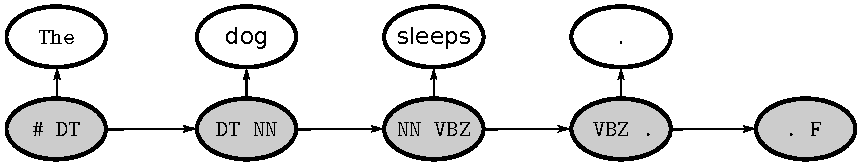
\includegraphics[scale=.7]{snd_order_path}
\caption{A second order HMM for a sentence.}\label{second-order-fig}
\end{center}
\end{figure}

The example with adverbs is poor at best, but it illustrates the kind
of effect {\it second order} information can have. Second order HMMs
are models where transitions are conditioned on two preceding hidden
states. Equivalently, in POS tagging, the hidden states can be taken
to be pairs of POS tags, e.g. {\tt (DT, NN)}. In such a model
transitions can only occur to a subset of the hidden state set. For
example a transition from {\tt (DT, NN)} to {\tt (NN, VBZ)} is possible,
but a transition to {\tt (JJ, NN)} is impossible. Figure
\ref{second-order-fig} illustrates a path with legal transitions. 

Figure \ref{second-order-fig} implies that emissions in a second order
model are conditioned on two labels like the transitions. However,
many existing HMM based POS tagging systems such as \cite{Brants2000}
condition emissions only on one label, that is use $e_{t_i, t_{i -
    1}}(w_i) = p(w_i \cond t_i)$ instead of $e_{t_i, t_{i - 1}}(w_i) =
p(w_i \cond t_{i - 1},\ t_{i})$. The reason is probably
data-sparsity. Therefore, these systems cannot be called HMMs in the
strictest sense of the word. They should instead be called trigram
taggers. 

\cite{Halacsy2007}, show that it is possible to maintain the correct
HMM formulation over-come the data sparseness problem and achieve
gains over the more commonly used trigram tagger. However, they fail
to describe the smoothing scheme used, which is crucial. This defect
is partly remedied by the fact that the system is open-source.  One of
the chief contributions of Publication \ref{pub:2} was to investigate
the effect of different ways of estimating the emission parameters in
a generative trigram tagger paying attention to smoothing.
 
Increasing model order unfortunately leads to increased data sparsity
because the number of hidden states increases. Therefore, smoothing
transition probabilities is even more important than in the first
order case. %Even using smoothing, third and higher order models tend
%to generalize to unseen data more poorly than lower order models
%because of over-fitting \citep{foo}.

An alternative to increasing model order, is to use so called latent
annotations \citep{Huang2009} in an otherwise regular first order
HMM. Conceptually, each label for example {\tt NN} is split into a
number of sub-states {\tt NN1}, {\tt NN2} and so on. Expectation
maximization is used to train the model in a partly supervised
fashion. Splitting labels, and indeed any increase in order, is
probably works better for label sets with quite few labels. Otherwise,
it will simply contribute to data sparsity.

%\section{HMMs for POS Tagging}

\section{HMM taggers and Morphological Analyzers}
\label{sec:hmm-label-dict}
%\begin{itemize}
%\item Limiting transitions.
%\item How much of an improvement can be expected?
%\end{itemize}

The inventory of POS labels that are possible for a given word form
tends to be small. For example the English ``dog'' can get two of the
Penn Treebank POS tags singular noun {\tt NN} and {\tt VB} infinitive
verb form. The remaining 43 POS tags can never label
``dog''. Consequently, in an HMM POS tagger, only the states
corresponding to {\tt VB} and {\tt NN} should ever emit the word
``dog''.

A {\tt tag dictionary} \citep{Brants2000} can be used in combination
with the Viterbi algorithm to limit the set of hidden states that
could emit a word. The tag dictionary can be constructed from the
training corpus. Additionally, an external lexical resource, such as a
morphological analyzer, can be used. Such a lexical resource can help
to compensate for missing statistics for OOV words. In the frequent
setting, where most rare words have quite few analyses, this can have
a substantial effect on tagging accuracy.

